\documentclass{ctexart}
\usepackage{avanti-color}
%\usepackage{avanti-font}
\usepackage{avanti-math}
\usepackage{avanti-theorem}
\usepackage{avanti-others}

\RequirePackage{fontspec}
\xeCJKsetup{CJKmath=true}
\setCJKmainfont[BoldFont=FZHei-B01,ItalicFont=]{LXGW Bright}

\everymath{\color{Solarized-magenta}}
\pagestyle{empty} % 没有页眉和页脚

\tikzset{font=\Large}
\tikzset{base/.style={smooth, very thick, Solarized-base01}}
\tikzset{arrow/.style={->, -{Stealth[scale=1.0]}, base}}
\tikzset{point/.style={circle, fill, inner sep=1.5pt, Solarized-base01}}

\begin{document}

\begin{figure}[htbp]
    \centering
    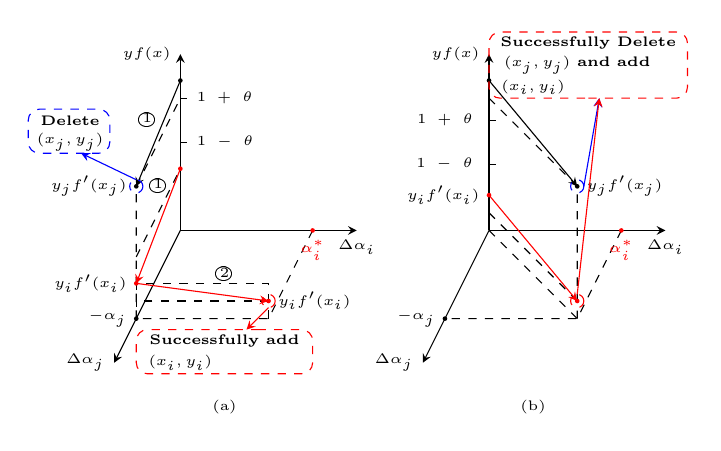
\begin{tikzpicture}[font = \tiny ,scale = 0.28]
        \tikzset{global scale/.style={
                    scale=#1,
                    every node/.append style={scale=#1}
                }
        }
        % 坐标轴
        \draw[->,>=stealth,scale = 1.0] (0,0) -- (8,0) node () [below] {$\Delta \alpha_i$};
        \draw[->,>=stealth,scale = 1.0] (0,0) -- (0,8) node () [left] {$yf(\bm{x})$};
        \draw[->,>=stealth,scale = 1.0] (0,0) -- (-3,-6) node () [left] {$\Delta \alpha_j$};

        %虚线
        \draw[dashed] (6,0) -- ++(-2,-4) -- (-2,-4);
        \draw[dashed] (4,-4) -- ++(0,1.6) -- (-2,-2.4) -- ++(0,-1.6);
        \draw[dashed] (4,-3.2) -- (-2,-3.2);
        \draw[dashed] (-2,-4) -- (-2,2) -- ++(2,4);
        \draw[dashed] (-2,-1.2) -- ++(2,4);

        %描点
        \fill [red] (6,0) circle (3pt) node () [below] {$\alpha_i^*$};
        \node at (4,-3.2) [right] {$y_if^\prime(\bm{x}_i)$};
        \fill [red] (0,2.8) circle (3pt);
        \fill (-2,-4) circle (3pt) node () [left] {$-\alpha_j$};
        \node at (-2,-2.4) [left] {$y_if^\prime(\bm{x}_i)$};
        \fill (0,6.8) circle (3pt);
        \draw (0,6) -- ++(0.3,0) node () [right] {$1 \ + \ \theta$};
        \draw (0,4) -- ++(0.3,0) node () [right] {$1 \ - \ \theta$};
        \fill [red] (-2,-2.4) circle (3pt);
        \fill [red] (4,-3.2) circle (3pt);
        \fill (-2,2) circle (3pt) node () [left] {$y_jf^\prime(\bm{x}_j)$};

        %箭头
        \draw [->,>=stealth,scale = 1.0] (0,6.8) -- (-2,2);
        \draw [->,>=stealth,scale = 1.0,red] (0,2.8) -- (-2,-2.4);
        \draw [->,>=stealth,scale = 1.0,red] (-2,-2.4) -- (4,-3.2);

        %圆圈
        \node at (-1.5,5) {$\textcircled{1}$};
        \node at (-1,2) {$\textcircled{1}$};
        \node at (2,-2) {$\textcircled{2}$};

        %文字
        \draw [dashed,blue] (-2,2) circle (0.3);
        \draw [->,>=stealth,scale = 1.0,blue] (-2,2.3) -- (-4.5,3.5);
        \node at (-5,5) {${\rm \mathbf{Delete}}$};
        \node at (-5,4) {$(\bm{x}_j,y_j)$};
        \draw[dashed,rounded corners,blue] (-4.5,3.5) -- ++ (1.3,0) -- ++(0,2) -- ++(-3.7,0) -- ++(0,-2) -- cycle;

        \draw [dashed,red] (4,-3.2) circle (0.3);
        \draw [->,>=stealth,scale = 1.0,red] (4,-3.5) -- (3,-4.5);
        \node at (2,-5) {${\rm \mathbf{Successfully \ add }}$};
        \node at (0,-6) {$(\bm{x}_i,y_i)$};
        \draw[dashed,rounded corners,red] (3,-4.5) -- ++ (3,0) -- ++(0,-2) -- ++(-8,0) -- ++(0,2) -- cycle;

        %标签(伪)
        \node at (2,-8) {(a)};

        \pgfmathsetmacro{\offset}{14};
        %第二幅图
        \draw[->,>=stealth,scale = 1.0] (0 + \offset,0) -- ++(8,0) node () [below] {$\Delta \alpha_i$};
        \draw[->,>=stealth,scale = 1.0] (0 + \offset,0) -- ++(0,8) node () [left] {$yf(\bm{x})$};
        \draw[->,>=stealth,scale = 1.0] (0 + \offset,0) -- ++(-3,-6) node () [left] {$\Delta \alpha_j$};

        %虚线
        \draw[dashed] (6 + \offset,0) -- ++(-2,-4) -- (-2 + \offset,-4);
        \draw[dashed] (0 + \offset,0) -- (4  + \offset,-4);
        \draw[dashed] (0 + \offset,6) -- (4 + \offset,2) -- (4 + \offset,-4);
        \draw[dashed] (0 + \offset,0.8) -- ++(4,-4);

        %描点
        \fill [red] (6 + \offset,0) circle (3pt) node () [below] {$\alpha_i^*$};
        \fill [red] (0 + \offset,1.6) circle (3pt);
        \fill [red] (4 + \offset,-3.2) circle (3pt);
        \fill (-2 + \offset,-4) circle (3pt) node () [left] {$-\alpha_j$};
        \fill (4 + \offset,2) circle (3pt);
        \node at (4 + \offset,2) [right] {$y_jf^\prime(\bm{x}_j)$};
        \node at (0 + \offset,1.6) [left] {$y_if^\prime(\bm{x}_i)$};
        \fill (0 + \offset,6.8) circle (3pt);
        \draw (0 + \offset,5) -- ++(0.3,0) ++(-0.6,0) node () [left] {$1 \ + \ \theta$};
        \draw (0 + \offset,3) -- ++(0.3,0) ++(-0.6,0) node () [left] {$1 \ - \ \theta$};

        %箭头
        \draw [->,>=stealth,scale = 1.0] (0 + \offset,6.8) -- ++(4,-4.8);
        \draw [->,>=stealth,scale = 1.0,red] (0 + \offset,1.6) -- ++(4,-4.8);

        %文字
        \draw [dashed,blue] (4 + \offset,2) circle (0.3);
        \draw [->,>=stealth,scale = 1.0,blue] (4.3 + \offset,2) -- (5 + \offset,6);
        \node at (4 + \offset,7.5) {$(\bm{x}_j,y_j) \ {\rm \mathbf{and \ add }}$};
        \node at (2 + \offset,6.5) {$(\bm{x}_i,y_i)$};
        \node at (4.5 + \offset,8.5) {${\rm \mathbf{Successfully \ Delete}}$};
        \draw[dashed,rounded corners,red] (4 + \offset,6) -- ++ (5,0) -- ++(0,3) -- ++(-9,0) -- ++(0,-3) -- cycle;
        \draw [dashed,red] (4 + \offset,-3.2) circle (0.3);
        \draw [->,>=stealth,scale = 1.0,red] (4 + \offset,-2.9) -- (5 + \offset,6);

        %标签(伪)
        \node at (2 + \offset,-8) {(b)};
    \end{tikzpicture}
\end{figure}

\end{document}
